\documentclass[a4paper,twoside]{article}
\usepackage{fancyhdr}
\usepackage{pdfpages}
\usepackage[a4paper,inner=3cm,outer=2 cm,bottom=3cm,top=2cm]{geometry}
\usepackage{multicol,verse}
\usepackage[doublespacing]{setspace}
\usepackage{tocloft}
\usepackage[hidelinks]{hyperref}

\renewcommand\cftsecleader{\cftdotfill{\cftdotsep}}
\renewcommand\cftbeforesecskip{-1 pt}

\date{\vspace{-12ex}}


\setlength{\footskip}{2 cm}

%%CHANGE OFFSET to 5mm for printing (offset moves towards outside of page):
\newcommand*{\offset}{5mm}
\newcommand*{\addsong}[2]{
\phantomsection
\addcontentsline{toc}{section}{#1}
\includepdf[pages=-,pagecommand={\thispagestyle{plain}},scale=0.95,offset=\offset{} 0mm]{./SongFiles/#2.pdf}}


\begin{document}
%
\includepdf[pages=-,pagecommand={\thispagestyle{empty}},scale=0.95,offset=\offset{} 0mm]{./BookCover/cover-print.pdf}
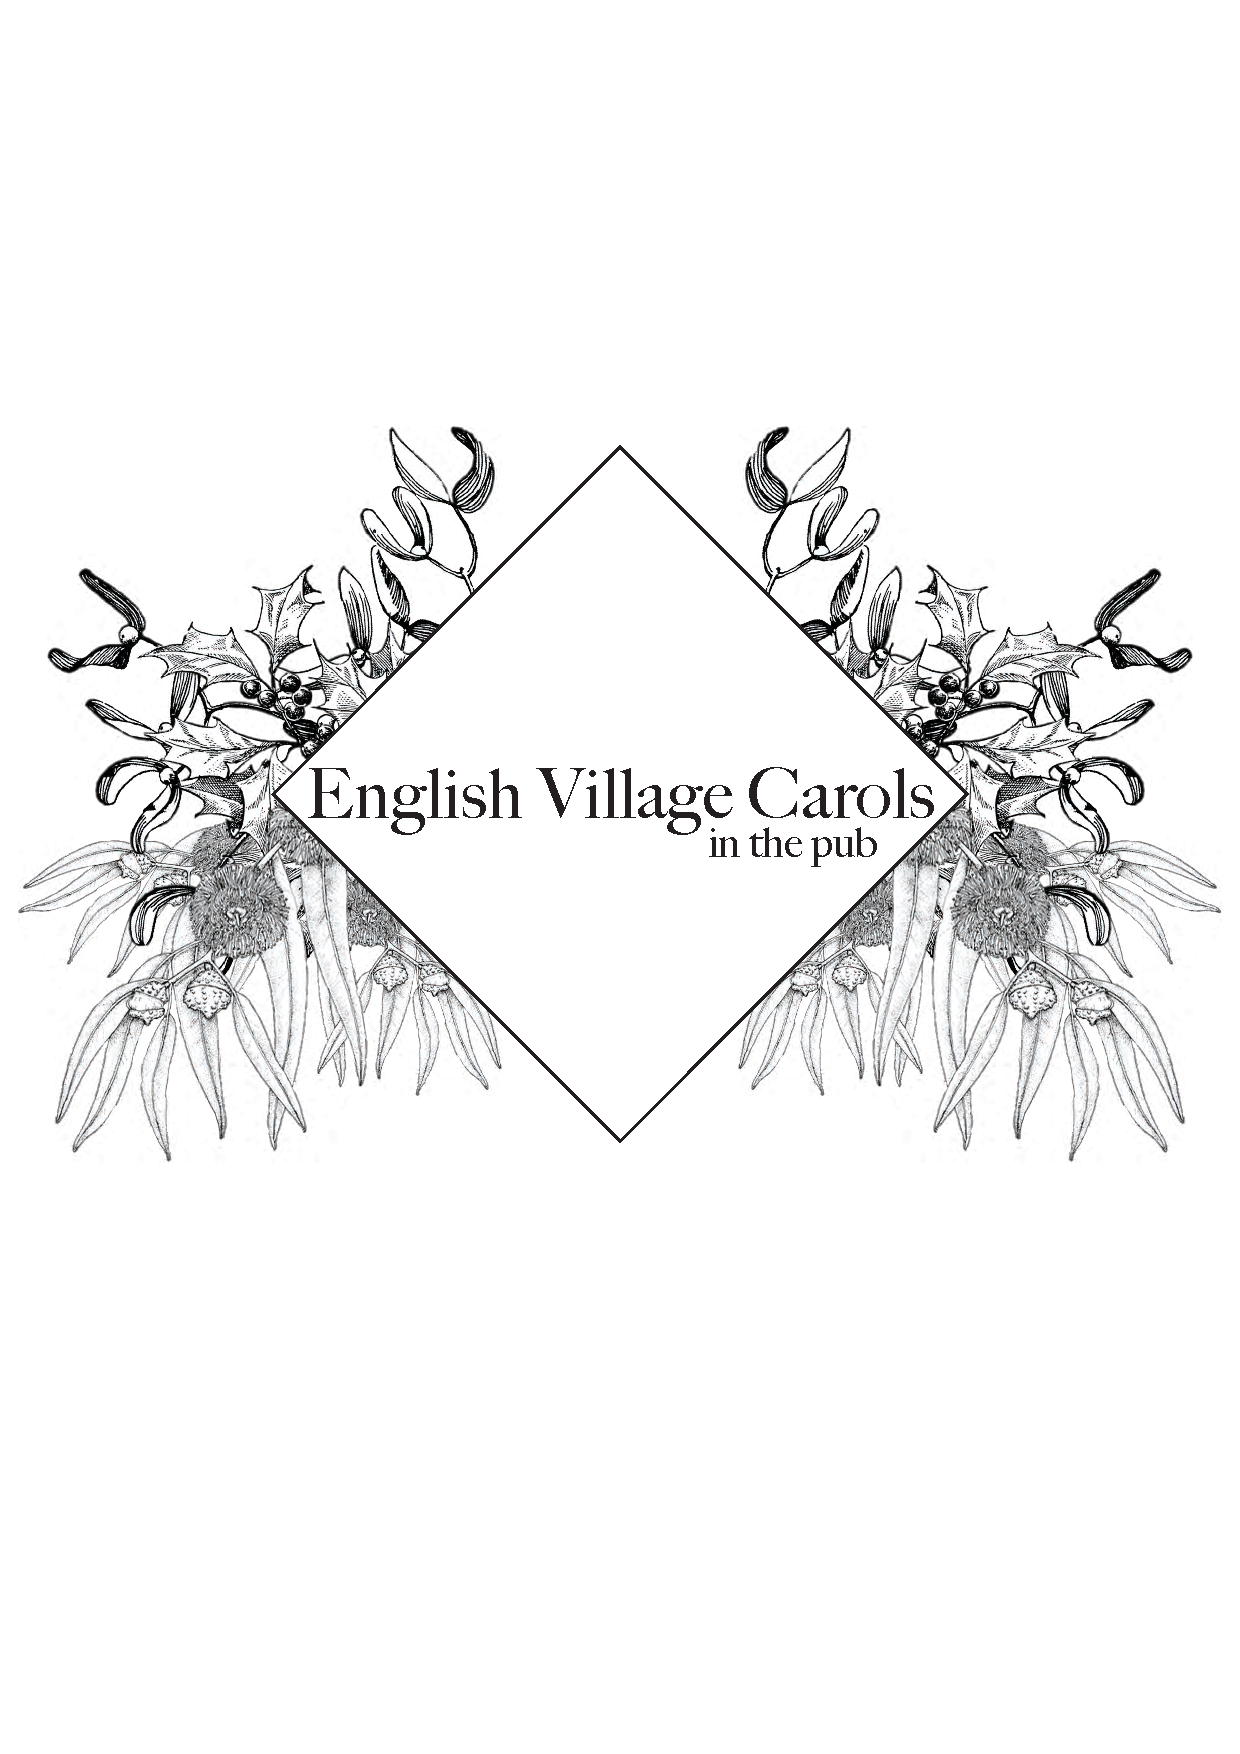
\includepdf[pages=-,pagecommand={\thispagestyle{empty}},scale=0.95,offset=\offset{} 0mm]{./BookCover/cover-webmed.pdf}
\clearpage

\thispagestyle{empty}
    \null\vspace{\stretch {1}}
        \begin{center}        
The arrangements in this book are generously shared by Ian Russell for use in Sydney. 

To support his work, we recommend The Sheffield Book of Village Carols: \url{http://www.villagecarols.org.uk/publications/sheffield-book.html}\\
and ask that you do not redistribute this songbook.\\


To keep up to date with carol-singings in Sydney, please join our Facebook group at \url{https://www.facebook.com/groups/VillageCarolsSydney/}\\

Music set by Thomas MacDonald in Lilypond and LaTeX. Cover art by Stephanie Swanson.
       \end{center}
\vspace{\stretch{1}}\null

\section*{Distributed versions of this book}
\subsection*{First printing (2018)}
\begin{itemize}
    \item 31 songs included, 52 pages.
    \item Song ordering largely alphabetical but with some fudging to keep 2-page songs on facing pages.
\end{itemize}
\subsection*{Second printing (2022)}
\begin{itemize}
    \item Multiple fixes of typos and incorrect word alignment below music.
    \item Song ordering changed to be fully alphabetical. 
    \item New songs: Reapers, Shepherds Arise, Stannington. 34 songs included, 60 pages.
\end{itemize} 
\clearpage


\tableofcontents
\setcounter{page}{1} %Set TOC as page 1: previous pages are the cover.
\clearpage
% TWo-page songs should begin on even page numbers (lefthand side) wherever possible.
\addsong{Awake and Arise}{awake_and_arise}

\addsong{Awake, Arise, Good Christians!}{awake_arise_good_christians}

\addsong{Back Lane}{back_lane}

\addsong{The Christmas Tree}{christmas_tree}

\addsong{Curly Hark}{curly_hark}

\addsong{Diadem}{diadem}

\addsong{Egypt}{Egypt}

\addsong{Good News}{good_news}

%\addsong{Hail! Chime on}{hail_chime_on  }

\addsong{Hail, Smiling Morn!}{hail_smiling_morn}

\addsong{Hark Hark, Hark Hark}{hark_hark}

\addsong{How Beautiful Upon The Mountains}{how_beautiful_upon_the_mountain}

\addsong{Jacob's Well}{jacobs_well}

\addsong{Little Bilberry}{little_bilberry}

\addsong{Liverpool}{liverpool}

\addsong{Lloyd}{lloyd}

\addsong{Lo, the Eastern Magi Rise}{lo_the_eastern_magi_rise}

\addsong{Malin Bridge}{malin_bridge}

\addsong{Merry Christmas}{merry_christmas}

\addsong{The Mistletoe Bough}{mistletoe_bough}

\addsong{Mount Moriah}{mount_moriah}

\addsong{Mount Zion}{mount_zion}

\addsong{Old Foster}{old_foster}

\addsong{Peace O'er the World}{peace_oer_the_world}

\addsong{Pentonville}{pentonville}

\addsong{Prodigal Son}{prodigal_son}

\addsong{Reapers}{ho_reapers}

\addsong{Rolling Downward}{rolling_downward}

\addsong{Shepherds Arise}{shepherds_arise}

\addsong{Shepherds Rejoice}{shepherds_rejoice}

\addsong{Spout Cottage}{spout_cottage}

\addsong{Stannington}{stannington}

\addsong{Star of Bethlehem}{star_of_bethlehem}

\addsong{Sweet Chiming Bells}{sweet_chiming_bells}

\addsong{Tinwood}{tinwood}



\end{document}

